\chapter{Methods}
\section{Dataset}
The dataset was created by Dr. Tichy and his team using the Computer Vision Annotation Tool (CVAT). It has been extended and improved multiple times over the course of this work, and there is still ongoing work. At the time of writing this report, it consisted of 2599 bitewing X-ray images with 4575 annotations of tooth decay. Out of those, there are 890 images without any decay. The distribution of dental caries per image is depicted in the figure \ref{fig:hist_caries_per_img}. For clarity reasons, we omitted 6 images that contained more than 10 caries. From the histogram on the figure \ref{fig:hist_caries_dim}, we observe that most of the caries have dimensions between 10 and 75 pixels. However, there are outliers as big as 380 pixels per dimension. This diversity is increasing the difficulty of the task.

We used the COCO data-format to store data, and used the format during the whole work only with rare exceptions when custom data-format was needed. During the experiments, we used the 70:15:15 split into training, validation and test dataset.
\begin{figure}
    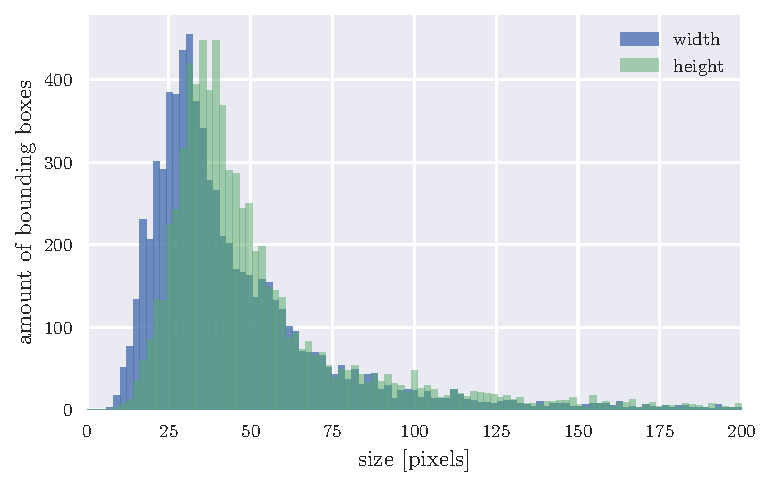
\includegraphics[width = \linewidth]{images/dataset_histogram.pdf}
    \caption{Histogram of bonding boxes dimensions in the dataset}
    \label{fig:hist_caries_dim}
\end{figure}

\begin{figure}
    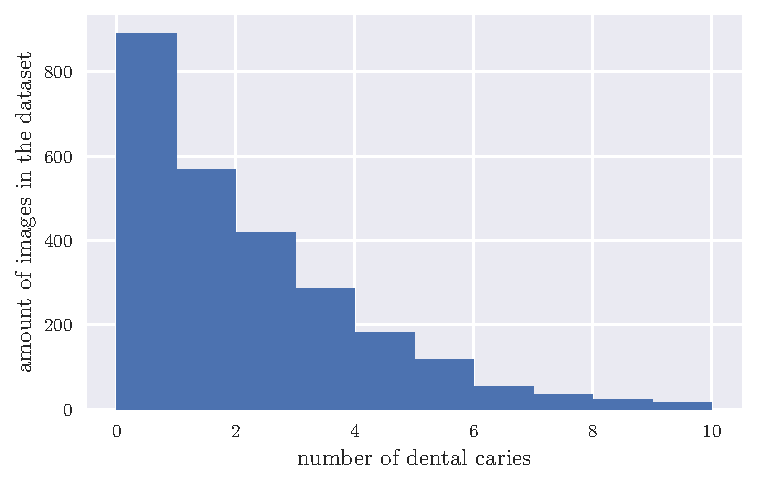
\includegraphics[width=\linewidth]{images/caries_histogram.pdf}
    \caption{Histogram of the amount of dental caries per image}
    \label{fig:hist_caries_per_img}
\end{figure}

\section{Neural network models}